\label{sec:4.2}

%%%%%%%%%%%%%%%%%%%%%%%%%%%%%%%%%%%%%%%%%%%%%%%%%%%%%%%
% Static Linearity (INL, DNL) 
%%%%%%%%%%%%%%%%%%%%%%%%%%%%%%%%%%%%%%%%%%%%%%%%%%%%%%%

To evaluate the Differential Nonlinearity (DNL) and Integral Nonlinearity (INL) of the ColdADC, a sine wave is applied to the single-ended input of the ColdADC. The resulting ADC code density histograms are used to extract DNL and INL. Some representative distributions at LN$_2$ temperature are shown in Figure~\ref{fig:adc_inldnl}.

\begin{figure}[htb]
\centering
%\begin{minipage}[b]{1.0\textwidth}                                                                                                                    
\begin{center}
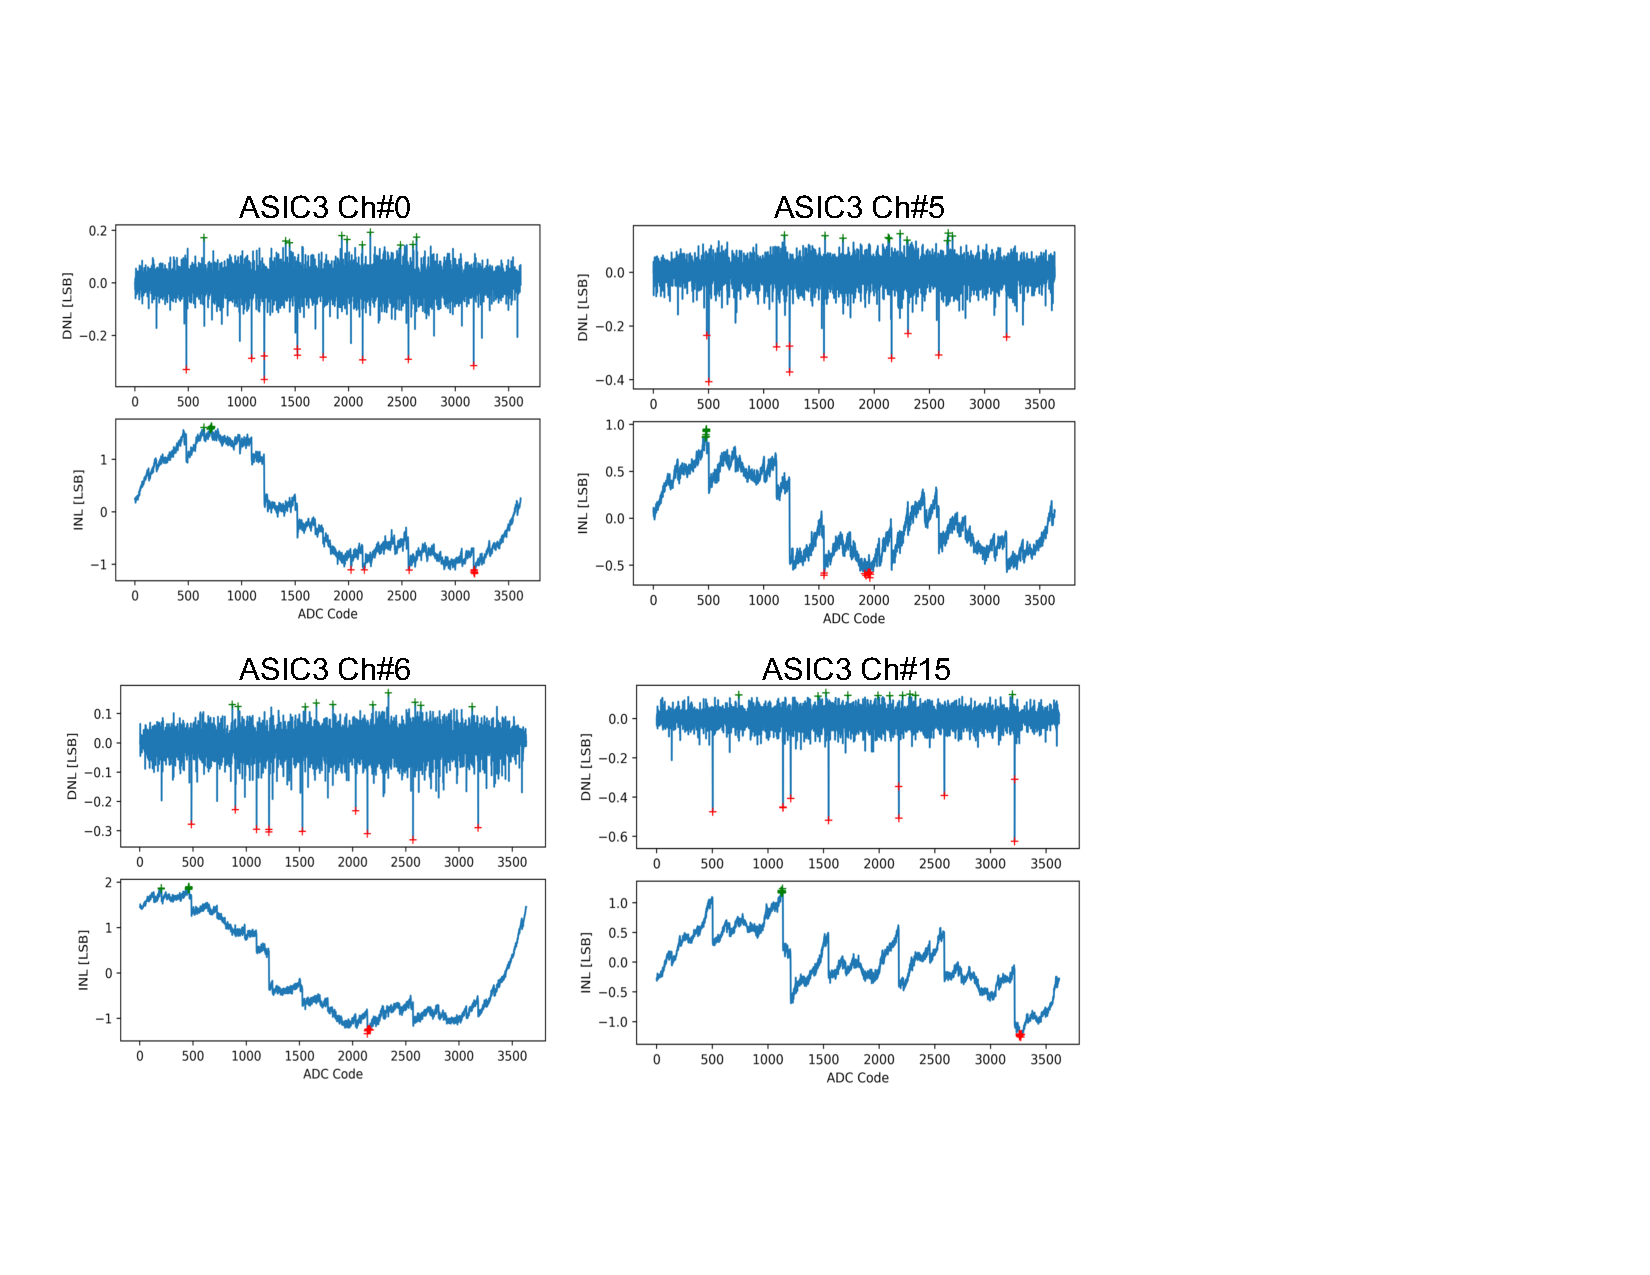
\includegraphics[width=1.0\textwidth]{figures/ColdADC_StaticLinearity.pdf}
\end{center}
%\end{minipage}                                                                                                                                        
\caption{DNL and INL for a few representative channels on ColdADC ASIC\#3 at LN$_2$ temperature.}
\label{fig:adc_inldnl}
\end{figure}

The typical DNL vs. ADC code has a narrow band between $\pm 0.1$ (12-bit) but exibits large negative spikes. The source of the spikes are attributed to residual nonlinearity from the MUX-SHA stage (to be discussed in Section~\ref{sec:5.4}). The DNL extremas, dominated by the spikes, across all channels are typically between $+0.2$ to $-0.5$ LSB. The average INL extremas are from $+1.2$ to $-1.1$ LSB.


